% !TeX encoding = UTF-8
% !TeX spellcheck = es_ES
% !TeX root = CBus.tex
%!TEX root=CBus.tex
C-Bus es un standard LCB usado y promocionado por MERG\copyright. A bajo nivel utiliza un Bus CAN como transporte fisico de datos entre modulos (electronicos).

La idea de despligue es usar una topolgia de bus:
\begin{figure}[H]
    \centering
    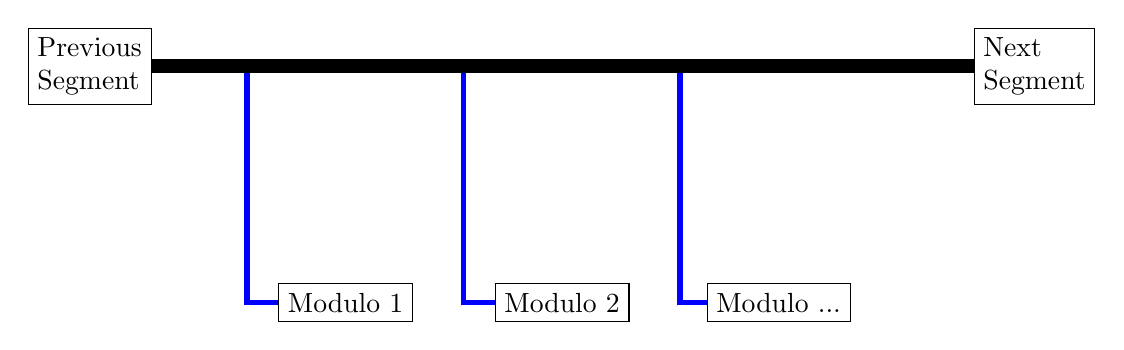
\begin{tikzpicture}
        %\draw [very thin, green]  (-6,-3) grid (6,3);
        \node at (-6,3) [rectangle,draw,align=left] (ps) {Previous\\Segment};
        \node at (6,3) [rectangle,draw,align=left] (ns) {Next\\Segment};
        
        \node at (-2.75,0) [rectangle,draw,align=left] (d1) {Modulo 1};
        \node at (0,0) [rectangle,draw,align=left] (d2) {Modulo 2};
        \node at (2.75,0) [rectangle,draw,align=left] (d3) {Modulo ...};

        \draw [line width=2px, blue] (-4,3) -- (-4,0) --(d1.west);
        \draw [line width=2px, blue] (-1.25,3) -- (-1.25,0) --(d2.west);
        \draw [line width=2px, blue] (1.5,3) -- (1.5,0) --(d3.west);

        \draw [line width=5px] (ps.east) -- (ns.west);
    \end{tikzpicture}
    \caption{C-Bus Segmento}
    \label{fig:cBusSegment}
\end{figure}

Al final de un segmento puede haber otro segmento, un repetidor, un convertidor a Ethernet,\dots.
Desde el bus a los dispositivos es necesario tener un latiguillo.


